\documentclass[class=report, crop=false, 12pt,a4paper]{standalone}
\usepackage{enumitem}
\usepackage{multicol}
\usepackage{etoolbox}
\AtBeginEnvironment{quote}{\singlespacing\small}
\usepackage{setspace}
\onehalfspacing
\usepackage{graphicx}
\usepackage{siunitx}
\sisetup{detect-all}
\begin{document}
\section{Fluid Properties}
Fluids have many properties including:

\begin{multicols}{2}
  \begin{itemize}[noitemsep]
    \item Surface Tension - \( \sigma \).
    \item Viscosity - \( \mu \).
    \item Compressibility.
    \item Density \( \rho \).
    \item Temperature.
    \item Pressure - P.
  \end{itemize}
\end{multicols}

What is a fluid?
\begin{quote}
  \begin{center}
    A fluid is a substance that deforms continuously when acted on by a shearing stress of any magnitude. 
  \end{center}
\end{quote}
This includes gases and liquids but not silly putty, gels or glass. Some soft materials such as toothpaste will only start to flow once a critical shear stress has been reached. This is the study of rheology and not studied in this module.

In classical fluid mechanics, we treat fluids as a continuum because there is an extremely large number of particles. Thus, we can conclude that fluid parameter such as pressure and density vary continously throughout the fluid.

\subsection{Shear strain for solid bodies}
What is shear strain?
\begin{quote}
  \begin{center}
    Shear strain is the change in angle as an element experience a force tangential to its surfave.
  \end{center}
\end{quote}
\begin{center}
  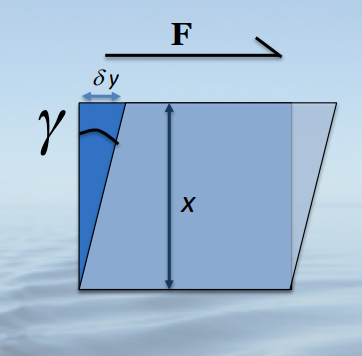
\includegraphics[width = 0.4 \textwidth]{../img/ShearStrainDiagram}
\end{center}
For a fluid, we are interested in the rate of shear. A specfic tangential force will caise a fixed amount of shear strain per unit time. If the speed of the top layer is \( u_y\), the shear rate is \(\delta u_y / \delta x\).
\begin{equation}
  tan(\gamma) = \frac{\delta y}{x} \approx \gamma
\end{equation}

\subsection{Shear Stress on a solid body}
For a solid, the shear force is the force applied tangentially to a surface.

\emph{Shear stress} is the tangential force per unit area \( \tau\).

\emph{Normal stress} is the perpendicular force per unit area \( \sigma \).

\begin{center}
  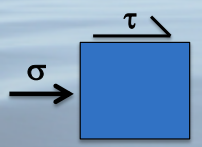
\includegraphics[width = 0.4 \textwidth]{../img/ShearForceDiagram}
\end{center}

\subsection{Simple laminar flow case}
Consider flat layers of fluid sliding over each other. The sideways velocity of the fluid changes as you move away from the stationary boundary. The velocity of the y direction, \( u_y \) is changing with position, \( x\). 

\begin{center}
  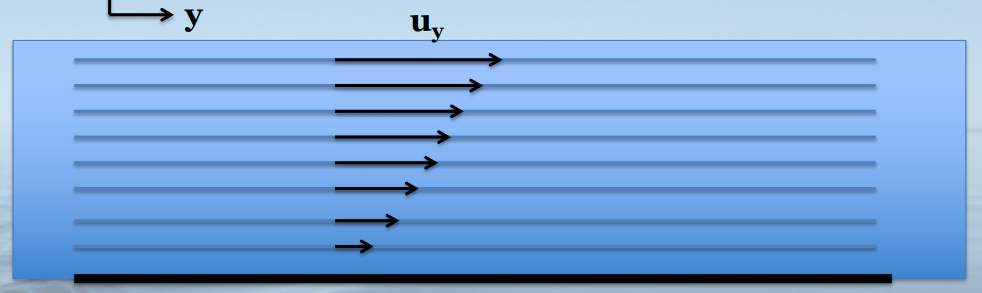
\includegraphics[width = 1 \textwidth]{../img/LaminarFlowSimple}
\end{center}

\subsection{Viscosity}
\begin{equation}
  \tau = \mu \frac{du_y}{dx}
\end{equation}
Where:
\begin{multicols}{2}
  \begin{itemize}[noitemsep]
    \item \(\tau \) = Shear stress = force/area.
    \item \(\mu \) = Dynamic viscosity.
    \item \( du_y / dx \) = Shear rate.
    \item Units: Velocity change per unit perpendicular distance.
  \end{itemize}
\end{multicols}
Viscosity is the constant of proportionality, telling us how much shear stress is required to produce a given shear rate. Shear stress can be different at different places in the same fluid. Equation (2) is Newton's equation for viscosity and he made the assumption that the viscosity was a constant. However, this is not always true and the fluids for which that does not apply are called \emph{non-Newtonian fluids.} An example of a shear \emph{thichekning} fluid is cornstarch, i.e. viscosity increases with shear rate. An example of shear \emph{thinning} fluid is blood or ketchup, i.e. viscosity decreases with shear rate. We cannot use laminar flow analysis to study blood vessels beacause they constrict and dilate as fluids pass through - the rigid boundary condition does not apply (or you would not be able to feel your pulse.) We will only be studying Newtonian fluids and rigid boundaries.

The standard symbol for the viscosity as defined above is \( \mu \) and this is known as the \emph{dynamic viscosity} with units \si{\kg\per\meter\per\second} or \si{\pascal \second}. This will be our definition of viscosity. For some applications it is easier to do calculations in terms of the viscosity per unit density:
\begin{equation}
  v = \frac{\mu}{\rho}
\end{equation}

\subsection{Surface tension}
\end{document}